% !TEX TS-program = pdflatex
% !TEX encoding = UTF-8 Unicode

% This file is a template using the "beamer" package to create slides for a talk or presentation
% - Giving a talk on some subject.
% - The talk is between 15min and 45min long.
% - Style is ornate.

% MODIFIED by Jonathan Kew, 2008-07-06
% The header comments and encoding in this file were modified for inclusion with TeXworks.
% The content is otherwise unchanged from the original distributed with the beamer package.

\documentclass{beamer}


% Copyright 2004 by Till Tantau <tantau@users.sourceforge.net>.
%
% In principle, this file can be redistributed and/or modified under
% the terms of the GNU Public License, version 2.
%
% However, this file is supposed to be a template to be modified
% for your own needs. For this reason, if you use this file as a
% template and not specifically distribute it as part of a another
% package/program, I grant the extra permission to freely copy and
% modify this file as you see fit and even to delete this copyright
% notice. 


\mode<presentation>
{
  \usetheme{Berkeley}
  % or ...

  \setbeamercovered{transparent}
  % or whatever (possibly just delete it)
}

\usepackage{tikz}
\usepackage{graphicx}
\usepackage[english]{babel}
% or whatever

\usepackage[utf8]{inputenc}
% or whatever

\usepackage{times}
\usepackage[T1]{fontenc}
% Or whatever. Note that the encoding and the font should match. If T1
% does not look nice, try deleting the line with the fontenc.


\title[Data Sharing and Replication] % (optional, use only with long paper titles)
{Data Sharing and Replication}

\subtitle
{Enabling Reproducible Research} % (optional)

\author[Christensen] % (optional, use only with lots of authors)
{Garret Christensen\inst{1}}
% - Use the \inst{?} command only if the authors have different
%   affiliation.

\institute[UC Berkeley, Berkeley Initiative for Transparency in the Social Sciences] % (optional, but mostly needed)
{
  \inst{1}%
  UC Berkeley: Berkeley Initiative for Transparency in the Social Sciences\\
  Berkeley Institute for Data Science
}
% - Use the \inst command only if there are several affiliations.
% - Keep it simple, no one is interested in your street address.

\date[Short Occasion] % (optional)
{New Delhi 2017}

\subject{Talks}
% This is only inserted into the PDF information catalog. Can be left
% out. 

\pgfdeclareimage[height=2cm]{university-logo}{../Images/BITSSlogo.png}
 \logo{\pgfuseimage{university-logo}}

% Delete this, if you do not want the table of contents to pop up at
% the beginning of each subsection:
%\AtBeginSubsection[]
%{
%  \begin{frame}<beamer>{Outline}
%   \tableofcontents[currentsection,currentsubsection]
%  \end{frame}
%}


% If you wish to uncover everything in a step-wise fashion, uncomment
% the following command: 

%\beamerdefaultoverlayspecification{<+->}

\begin{document}

% Since this a solution template for a generic talk, very little can
% be said about how it should be structured. However, the talk length
% of between 15min and 45min and the theme suggest that you stick to
% the following rules:  

% - Exactly two or three sections (other than the summary).
% - At *most* three subsections per section.
% - Talk about 30s to 2min per frame. So there should be between about
%   15 and 30 frames, all told.

\begin{frame}
  \titlepage
\end{frame}

\begin{frame}{Outline}
  \tableofcontents
  % You might wish to add the option [pausesections]
\end{frame}


\section{Introduction}
\begin{frame}{Reproducibility \& Transparency}
\begin{itemize}
\item What are problems associated with reproducibility?
\item What are solutions to these problems?
\item What are practical tools to implement these solutions?
\end{itemize}
\end{frame}
%%%%%%%%%%%%%%%%%%%%%%%%%%%%%%%%%%%%%%%%%%%%%%%%%%%%%%%%%%%%%%%%%%
\begin{frame}{Introduction}
Science advances by building on the work of others. 
\vspace{0.5in}


\begin{quote}
If I have seen further, it is by standing on the shoulders of giants
\end{quote}
\begin{flushright}
--Sir Isaac Newton, 1676
\end{flushright}
\end{frame}
%%%%%%%%%%%%%%%%%%%%%%%%%%%%%%%%%%%%

\begin{frame}{Problems}
What prevents us from building on others' work?
\begin{itemize}[<.->]
 \item Data not shared
 \item Analysis not shared
 \item Methods/protocol not shared 
\end{itemize}
\end{frame}

%%%%%%%%%%%%%%%%%%%%%%%%%%%%%%%%%%%%%%%
\begin{frame}{Solutions}
What enables us to build on others' work?
\begin{itemize}[<.->]
 \item Data shared in trusted public repository
 \item Code/Analysis shared in trusted public repository
 \item Methods/protocol follow appropriate reporting standard
 \item Also: findings/scholarly publications available (open access)
\end{itemize}
\end{frame}



%%%%%%%%%%%%%%%%%%%%%%%%%%%%%%%%%%%%%%%%%%%%%%%%%%%
\section{Project Protocol, Reporting Standards}
\begin{frame}[<.->]{Project Protocol, Reporting Standards}
 Make sure you report everything another researcher would need to replicate your research, including the exact methods.
 \pause
 
 What to report (following medicine):
\begin{itemize}
\item Find the appropriate reporting standard for your field and follow it.
\item Enhancing the QUAlity and Transparency Of health Research (\href{http://www.equator-network.org}{EQUATOR Network})
\item The most widely-adopted standard: \href{http://www.consort-statement.org}{Consolidated Standards of Reporting Trials (CONSORT)}. 
\item Standard Protocol Items: Recommendations for Interventional Trials (\href{http://www.spirit-statement.org}{SPIRIT Statement}).
\item Transparency and Openness Promotion (TOP) Guidelines: \url{http://cos.io/top}
\end{itemize}
\end{frame}

 { % all template changes are local to this group.
    \setbeamertemplate{navigation symbols}{}
    \begin{frame}[plain, label=AEAreg]
         \begin{tikzpicture}[remember picture,overlay]
            \node[at=(current page.center)] {
                
\includegraphics[width=\paperwidth]{../Images/TOPGuidelines.PNG}
            };
        \end{tikzpicture}
     \end{frame}
     
      \begin{frame}[plain, label=AEAreg]
         \begin{tikzpicture}[remember picture,overlay]
            \node[at=(current page.center)] {
                
\includegraphics[width=\paperwidth]{../Images/TakingUpTop.PNG}
            };
        \end{tikzpicture}
     \end{frame}
}

\begin{frame}{Project Protocol, Reporting Standards}
Where to report:

If not in the methods section of the article (of limited length), supplementary online appendix linked with article or in trusted digital repository.
\end{frame}
%%%%%%%%%%%%%%%%%%%%%%%%%%%%%%%%%%%%%%%%%%%%%%%%%%%%%%%%%%%%%%%%%%%%%%%
\section{Data Sharing}
\begin{frame}{Data Sharing}
\begin{itemize}
\item
To build on the work of others, data must be shared.
\item
Data sharing is associated with more citations (causality unclear). \href{http://journals.plos.org/plosone/article?id=10.1371/journal.pone.0000308}{Piwowar et al. 2007} 
\end{itemize}
\end{frame}
%%%%%%%%%%%%%%%%%%%%%%%%%%%%%%%%%%%%%%%%%%%%%%%%%%%%%

\begin{frame}{Data Sharing}
History in Economics:
\begin{itemize}
\item  \href{http://www.jstor.org/stable/1806061}{Journal of Money Credit and Banking Project}: Dewald, Thursby, Anderson \textit{AER} 1986. 
\begin{itemize}
\item Low response rate to requests to share data.
\item Attempted to reproduce 9 papers, problems with all (some minor) even with help of original authors.
\end{itemize}
\end{itemize}
\end{frame}


{ % all template changes are local to this group.
    \setbeamertemplate{navigation symbols}{}
    \begin{frame}[plain, label=AEAreg]
         \begin{tikzpicture}[remember picture,overlay]
            \node[at=(current page.center)] {
                
\includegraphics[width=\paperwidth]{../Images/JMCB1.PNG}
            };
        \end{tikzpicture}
     \end{frame}
    
    
    \begin{frame}[plain]
        \begin{tikzpicture}[remember picture,overlay]
            \node[at=(current page.center)] {
                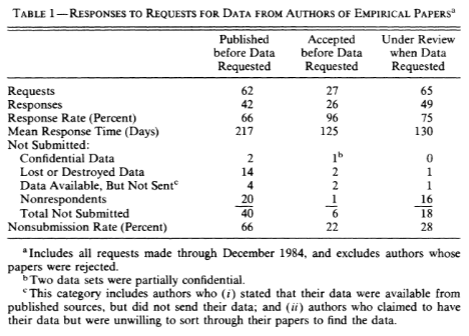
\includegraphics[width=\paperwidth]{../Images/JMCBTable1.PNG}
            };
        \end{tikzpicture}
     \end{frame}
}


%%%%%%%%%%%%%%
\begin{frame}{Data Sharing}
History in Economics:
\begin{itemize}
\item  \href{http://www.jstor.org/stable/1806061}{Journal of Money Credit and Banking Project}: Dewald, Thursby, Anderson \textit{AER} 1986. 
 \begin{itemize}
 \item Low response rate to requests to share data.
 \item Attempted to reproduce 9 papers, problems with all (some minor) even with help of original authors.
 \end{itemize}
\item \href{https://research.stlouisfed.org/publications/review/94/11/Replication_Nov_Dec1994.pdf}{A Decade After JMCB}: Anderson and Dewald, St Louis Fed 1994.
 \begin{itemize}
 \item Repeated similar experiment
 \item Similar bleak results
 \end{itemize}
 \pause
\item Verifying the Solution from a Nonlinear Solver, McCullough and Vinod, \textit{AER} 2003.
 \begin{itemize}
 \item Different software programs get you different answers.
 \item But finally change---\textit{AER} institutes data sharing requirement. \href{https://www.aeaweb.org/aer/data.php}{\beamerbutton{Policy}}
 \end{itemize} 
\end{itemize}
\end{frame}
%%%%%%%%%%%%%%


\begin{frame}{Data Sharing}
How is econ doing as a discipline?
\begin{itemize}
\item \textit{AER} internal review generally positive (\href{https://www.aeaweb.org/aer/2011_Data_Compliance_Report.pdf}{Glandon 2010})

\item Many, including McCullough, still skeptical of the ability to reproduce (\href{http://econjwatch.org/articles/got-replicability-the-journal-of-money-credit-and-banking-archive}{Econ Journal Watch, 2007})

\item Though \textit{AER}, all AEA, and other top 5 journals have mandatory data policies, and shared data is often only the ``analysis'' data instead of raw data. Exemptions for proprietary/restricted data increasing.

\item A study by the Replication Network shows that fewer than 27 journals regularly publish data, only 10 explicitly state they publish replications. (\href{http://econjwatch.org/articles/replications-in-economics-a-progress-report}{Duvendack et al 2015})

\end{itemize}
\end{frame}

%%%%%%%%%%%%%%%%%%%%%
{ % all template changes are local to this group.
    \setbeamertemplate{navigation symbols}{}
    \begin{frame}[plain, label=AEAreg]
         \begin{tikzpicture}[remember picture,overlay]
            \node[at=(current page.center)] {
                \includegraphics[width=\paperwidth]{../Images/ProprietaryDataGraphYEAR.png}
            };
        \end{tikzpicture}
     \end{frame}

}
%%%%%%%%%%%%%%%%%%%%%%



\begin{frame}{Data Sharing}
Why share your data in a trusted public repository?
\begin{itemize}[<.->]
\item
Find the appropriate repository: \url{http://www.re3data.org/}
\item
Repositories will last longer than your own website.
\item
Repositories are more easily searchable by other researchers.
\item
Repositories will store your data in a non-proprietary format that won't become obsolete.
\item 
Repositories manage meta-data better.
\item
Repositories create digital citable identifiers (DOI).

\end{itemize}
\end{frame}

\begin{frame}{Data Sharing}
Examples of Trusted Repositories:
\begin{itemize}
\item \href{http://dataverse.harvard.edu}{Harvard's Dataverse}
\item \href{http://datadryad.org/}{Data Dryad}
\item \href{http://figshare.com}{figshare}
\item \href{http://osf.io}{Open Science Framework}
\item \href{https://www.openicpsr.org/}{OpenICPSR} 
\item Check the journal--they may use one of these
\begin{itemize}
\item \href{https://dataverse.harvard.edu/dataverse/restat}{\textit{REStat}'s Dataverse}
\end{itemize}
\end{itemize}
\end{frame}

%\begin{frame}{ICPSR Repository}
%\begin{itemize}
%\item
%One of the longest run repositories, institutional member setup.
%\item
%New: \href{https://www.openicpsr.org/}{OpenICPSR} 
%\end{itemize}
%\end{frame}

%\begin{frame}{APHRC Repository}
%APHRC has created the APHRC Microdata Portal
%\begin{itemize}
%\item 30 Studies and growing
%\item \url{http://aphrc.org/catalog/microdata/index.php/catalog}
%\item Managed by Cheikh Faye
%\end{itemize}
%\end{frame}


%%%%%%%%%%%%%%%%%%%%%%%%%%%%%%%%%%%%%%
\section{Replication}
\begin{frame}{Replication}
\begin{itemize}
\item
With data available, we can begin to replicate studies.

\item 
We should be very careful about what we mean by ``replication.''

\item \href{http://www.cgdev.org/sites/default/files/CGD-Working-Paper-399-Clemens-Meaning-Failed-Replications.pdf}{``The Meaning of Failed Replications''} Michael Clemens, CGD Working Paper 399.
\end{itemize}
\end{frame}


{ % all template changes are local to this group.
    \setbeamertemplate{navigation symbols}{}
    \begin{frame}[plain]
        \begin{tikzpicture}[remember picture,overlay]
            \node[at=(current page.center)] {
                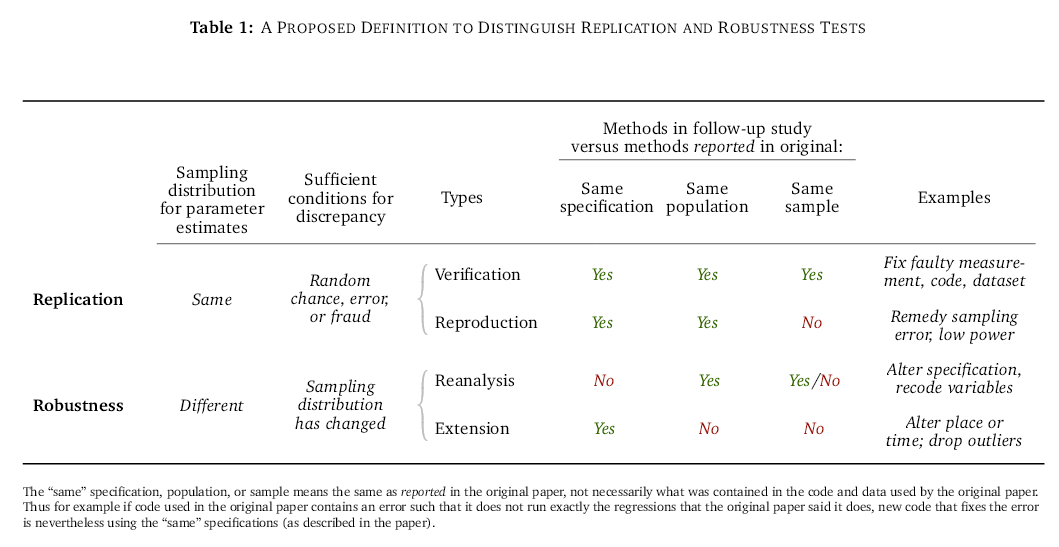
\includegraphics[width=\paperwidth]{../Images/ClemensReplication.PNG}
            };
        \end{tikzpicture}
     \end{frame}
}


\begin{frame}{Replication}
Why Replicate? \href{https://osf.io/ap6xz/}{Motivation} and suggestions from Nicole Janz of \href{https://politicalsciencereplication.wordpress.com/}{Political Science Replication} and Cambridge University
\begin{itemize}
\item For science in general:
\begin{itemize}\pause
\item Uncover misconduct and sloppy science
\item Confirm previous findings and generalizability
\item Point to misuse of statistical methods
\end{itemize}
\item For you as researchers:
\begin{itemize}\pause
\item Learn statistics
\item Jump to research frontier
\item Publish
\item Make your own research routinely reproducible
\item Fun
\end{itemize}
\end{itemize}
\end{frame}


\begin{frame}{Replication}
Which study should you pick to replicate? (Janz 2015)
\begin{itemize}
\item Don't select a study with methods that you don't know or can't learn within a reasonable time.
\item Pick a recent study (<5 yo) from a good journal.
\item Data (and code) should be publicly available.
\item The journal that published the original study has published replications before.
\end{itemize}
\end{frame}

\begin{frame}{Replication}
Which journals publish replications?
\begin{itemize}
\item List from \href{http://econjwatch.org/articles/replications-in-economics-a-progress-report}{The Replication Network study, Duvendack et al.}
\item Sadly fairly limtied in economics (10).
\item Selected journals from \href{https://osf.io/ap6xz/}{Janz (2015)}
\end{itemize}
\end{frame}

{ % all template changes are local to this group.
    \setbeamertemplate{navigation symbols}{}
    \begin{frame}[plain]
        \begin{tikzpicture}[remember picture,overlay]
            \node[at=(current page.center)] {
                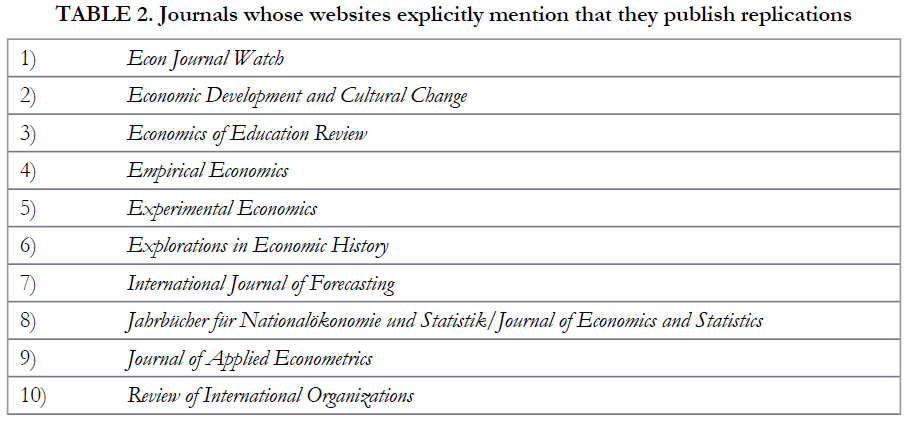
\includegraphics[width=\paperwidth]{../Images/DuvendackReplicationJournals.PNG}
            };
        \end{tikzpicture}
     \end{frame}

\setbeamertemplate{navigation symbols}{}
    \begin{frame}[plain]
        \begin{tikzpicture}[remember picture,overlay]
            \node[at=(current page.center)] {
                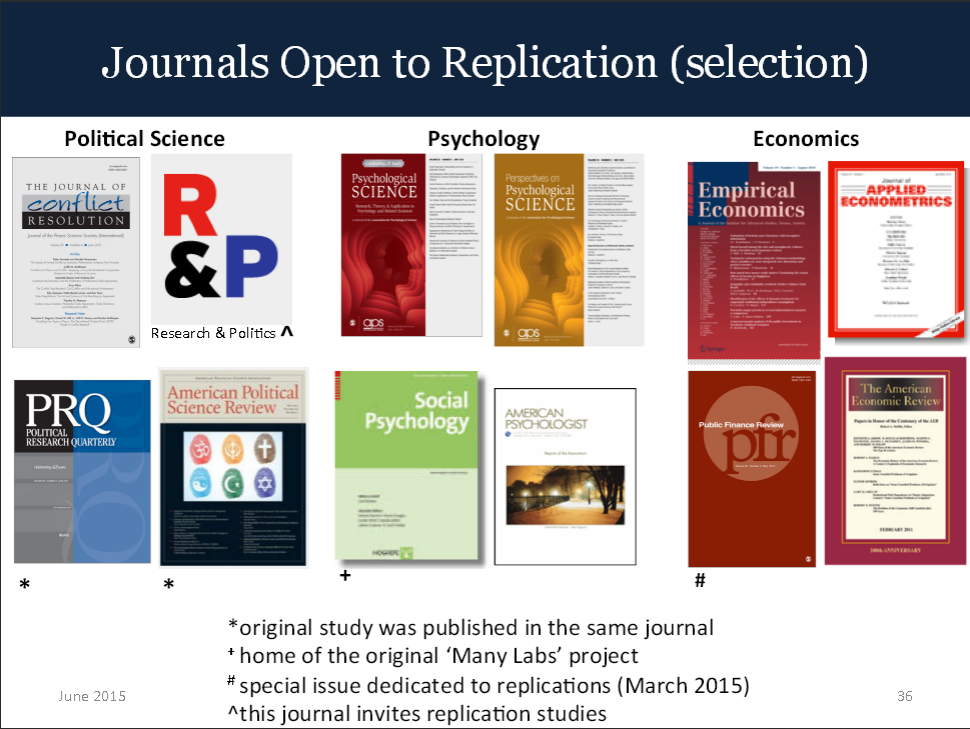
\includegraphics[width=\paperwidth]{../Images/JanzReplicationJournals.PNG}
            };
        \end{tikzpicture}
     \end{frame}
}

\begin{frame}{Replication}
How exactly to replicate?
\begin{itemize}
\item Be systematic: write a pre-analysis plan.
\item Don't just go on a fishing expedition. We all know that if you dig hard enough, you can find a specification that makes results appear weaker. Don't selectively report those specifications.
\item Be courteous and professional.
\item Take an entirely systematic approach:
\begin{itemize}
\item \href{https://osf.io/wx7ck/}{Many Labs Project}
\item \href{https://osf.io/gvm2z/}{Crowdsource your analysis}
\end{itemize}
\end{itemize}
\end{frame}

{ % all template changes are local to this group.
    \setbeamertemplate{navigation symbols}{}
    \begin{frame}[plain]
        \begin{tikzpicture}[remember picture,overlay]
            \node[at=(current page.center)] {
                \href{https://osf.io/wx7ck/}{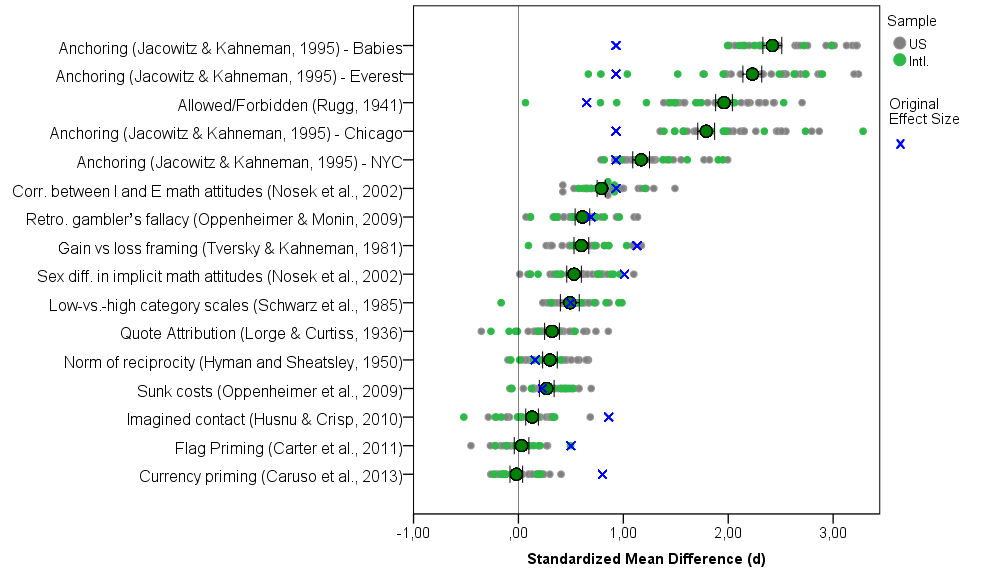
\includegraphics[width=\paperwidth]{../Images/ManyLabs.PNG}}
            };
        \end{tikzpicture}
     \end{frame}

\begin{frame}[plain]
        \begin{tikzpicture}[remember picture,overlay]
            \node[at=(current page.center)] {
                \href{https://osf.io/ezcuj/}{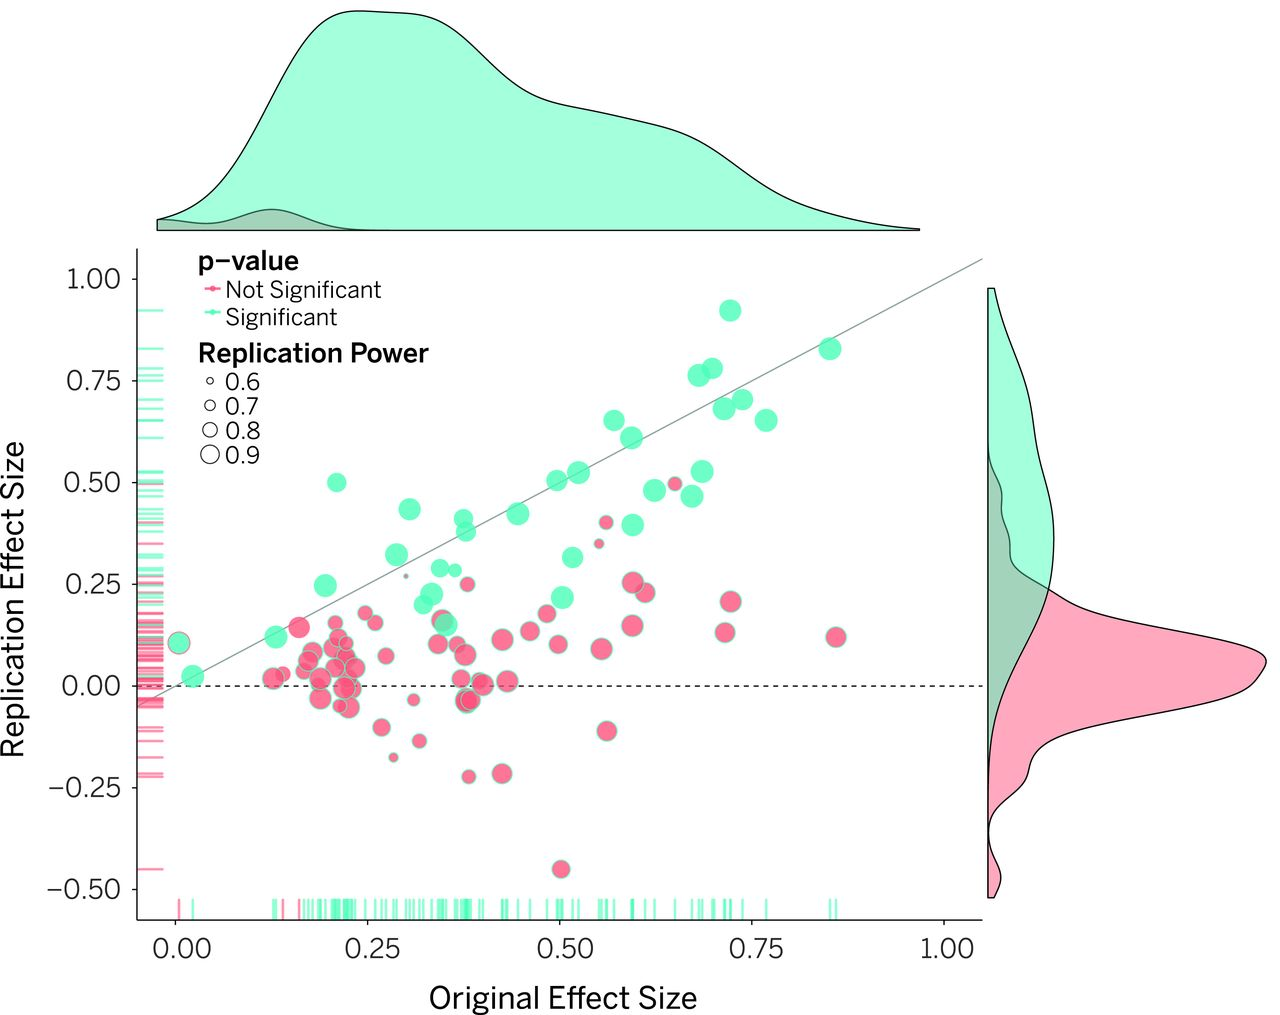
\includegraphics[height=\paperheight]{../Images/rpp.jpg}}
            };
        \end{tikzpicture}
     \end{frame}
     
\setbeamertemplate{navigation symbols}{}
    \begin{frame}[plain]
        \begin{tikzpicture}[remember picture,overlay]
            \node[at=(current page.center)] {
                \href{https://osf.io/gvm2z/}{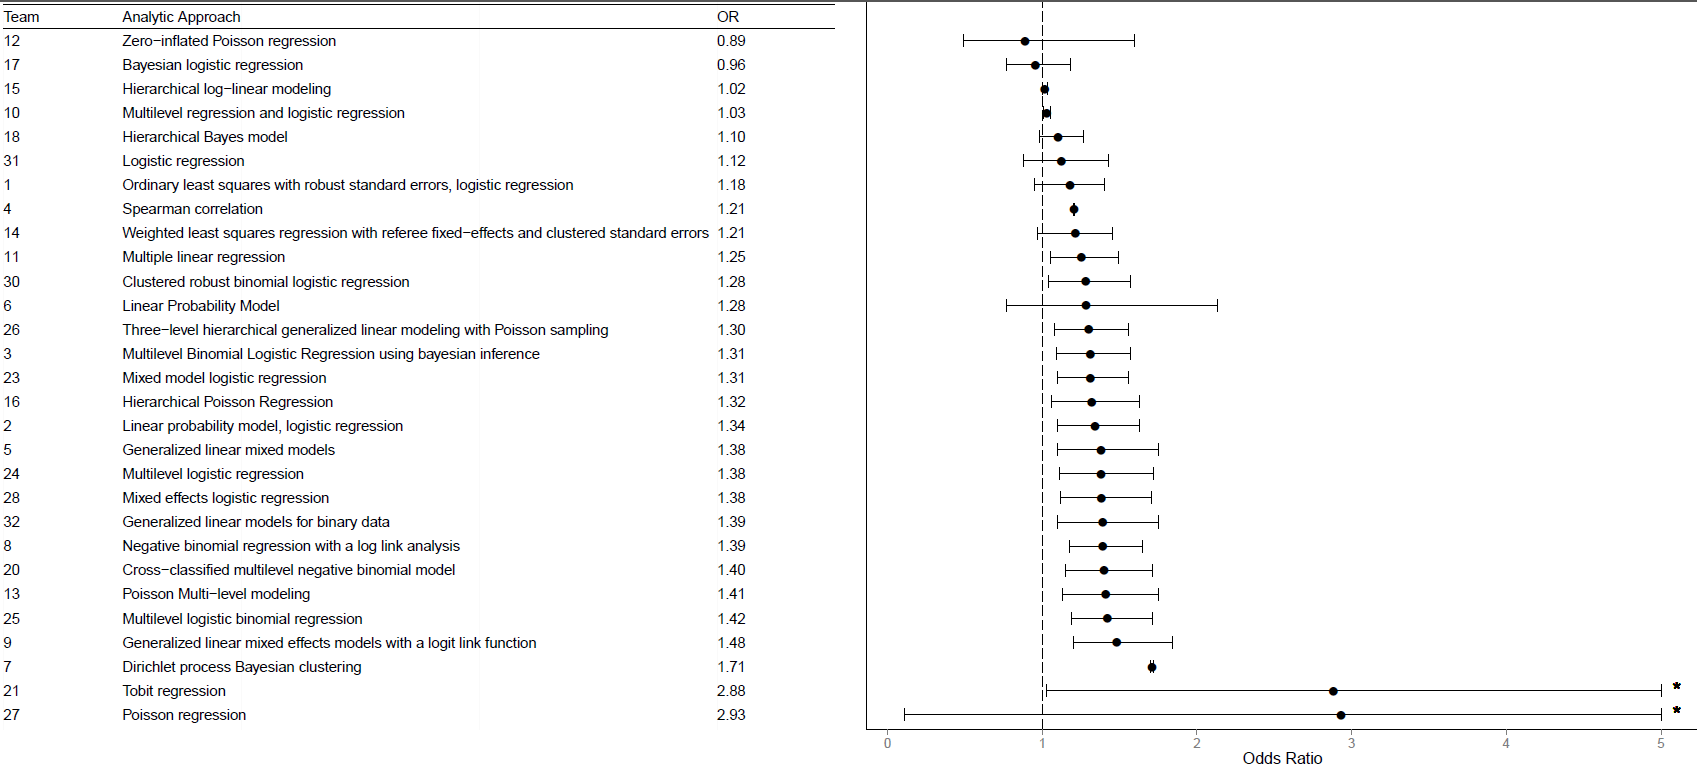
\includegraphics[width=\paperwidth]{../Images/Crowdsourcing.PNG}}
            };
        \end{tikzpicture}
     \end{frame}

    \begin{frame}[plain]
        \begin{tikzpicture}[remember picture,overlay]
            \node[at=(current page.center)] {
                \href{https://osf.io/gvm2z/}{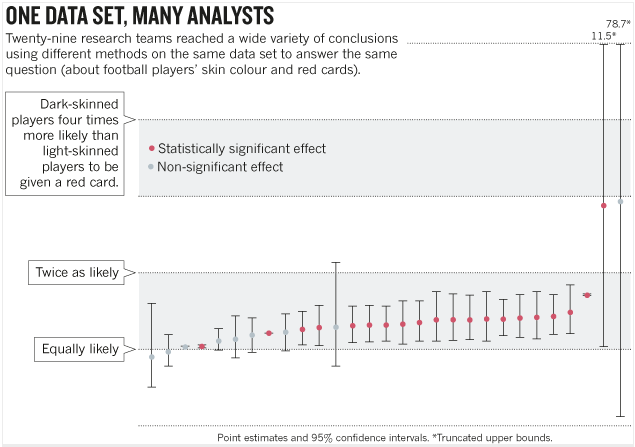
\includegraphics[width=\paperwidth]{../Images/Crowdsourcing2.PNG}}
            };
        \end{tikzpicture}
     \end{frame}
}

{ % all template changes are local to this group.
    \setbeamertemplate{navigation symbols}{}    
\begin{frame}[plain, label=AEAreg]
         \begin{tikzpicture}[remember picture,overlay]
            \node[at=(current page.center)] {
                \href{http://science.sciencemag.org/content/351/6280/1433}{
                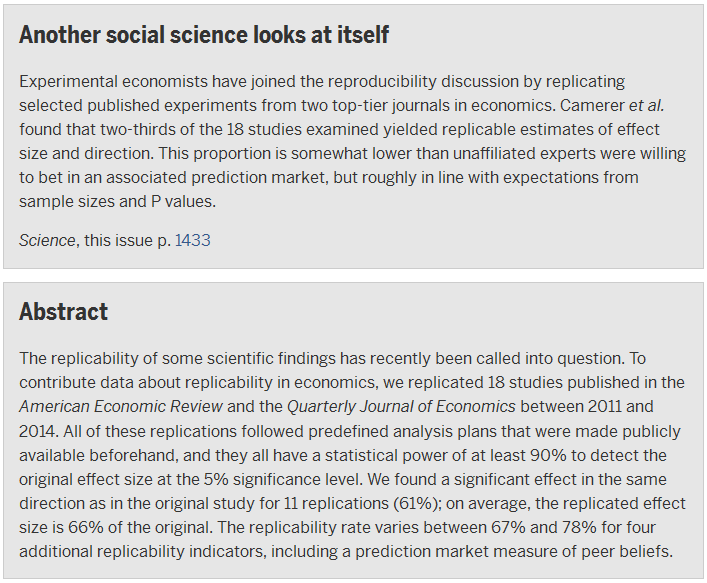
\includegraphics[height=\paperheight]{../Images/Camerer.PNG}}
            };
        \end{tikzpicture}
     \end{frame}

\begin{frame}[plain, label=AEAreg]
         \begin{tikzpicture}[remember picture,overlay]
            \node[at=(current page.center)] {
            	\href{http://www.sciencemag.org/news/2016/03/about-40-economics-experiments-fail-replication-survey}{
                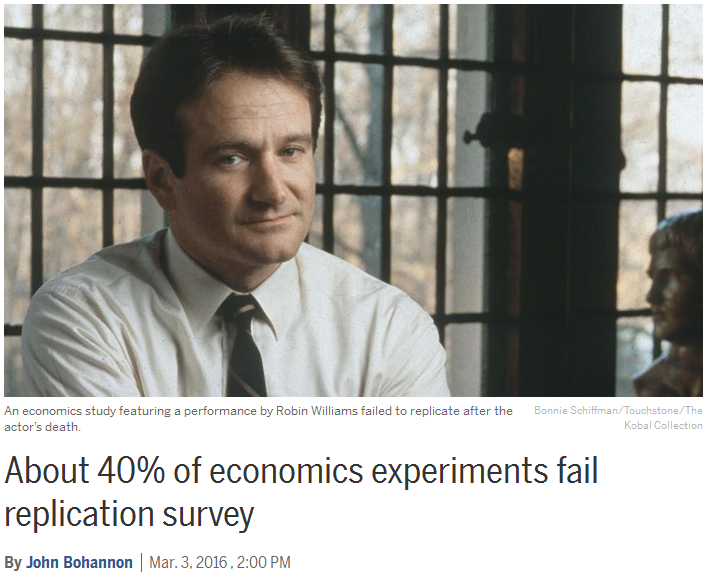
\includegraphics[height=\paperheight]{../Images/Bohannon.PNG}}
            };
        \end{tikzpicture}
     \end{frame}

}

%%%%%%%%%%%%%%%%%%%%%%%%%%%%%%%%%%%%%%
\section{Conclusion}
\begin{frame}{Conclusion}
\begin{itemize}
\item Science builds on previous work
\item To do that, work must be public
\item Share your data and code publicly
\item Replicate the work of others
\end{itemize}
\end{frame}

\end{document}


